\chapter{Metodologia}
\label{cap:metodologia}
Este capítulo apresenta a metodologia e os recursos utilizados para atingir o objetivo do trabalho.

\section{Visão geral}
\begin{figure}[h]
    \centering
    \caption{Etapas de desenvolvimento da pesquisa}
    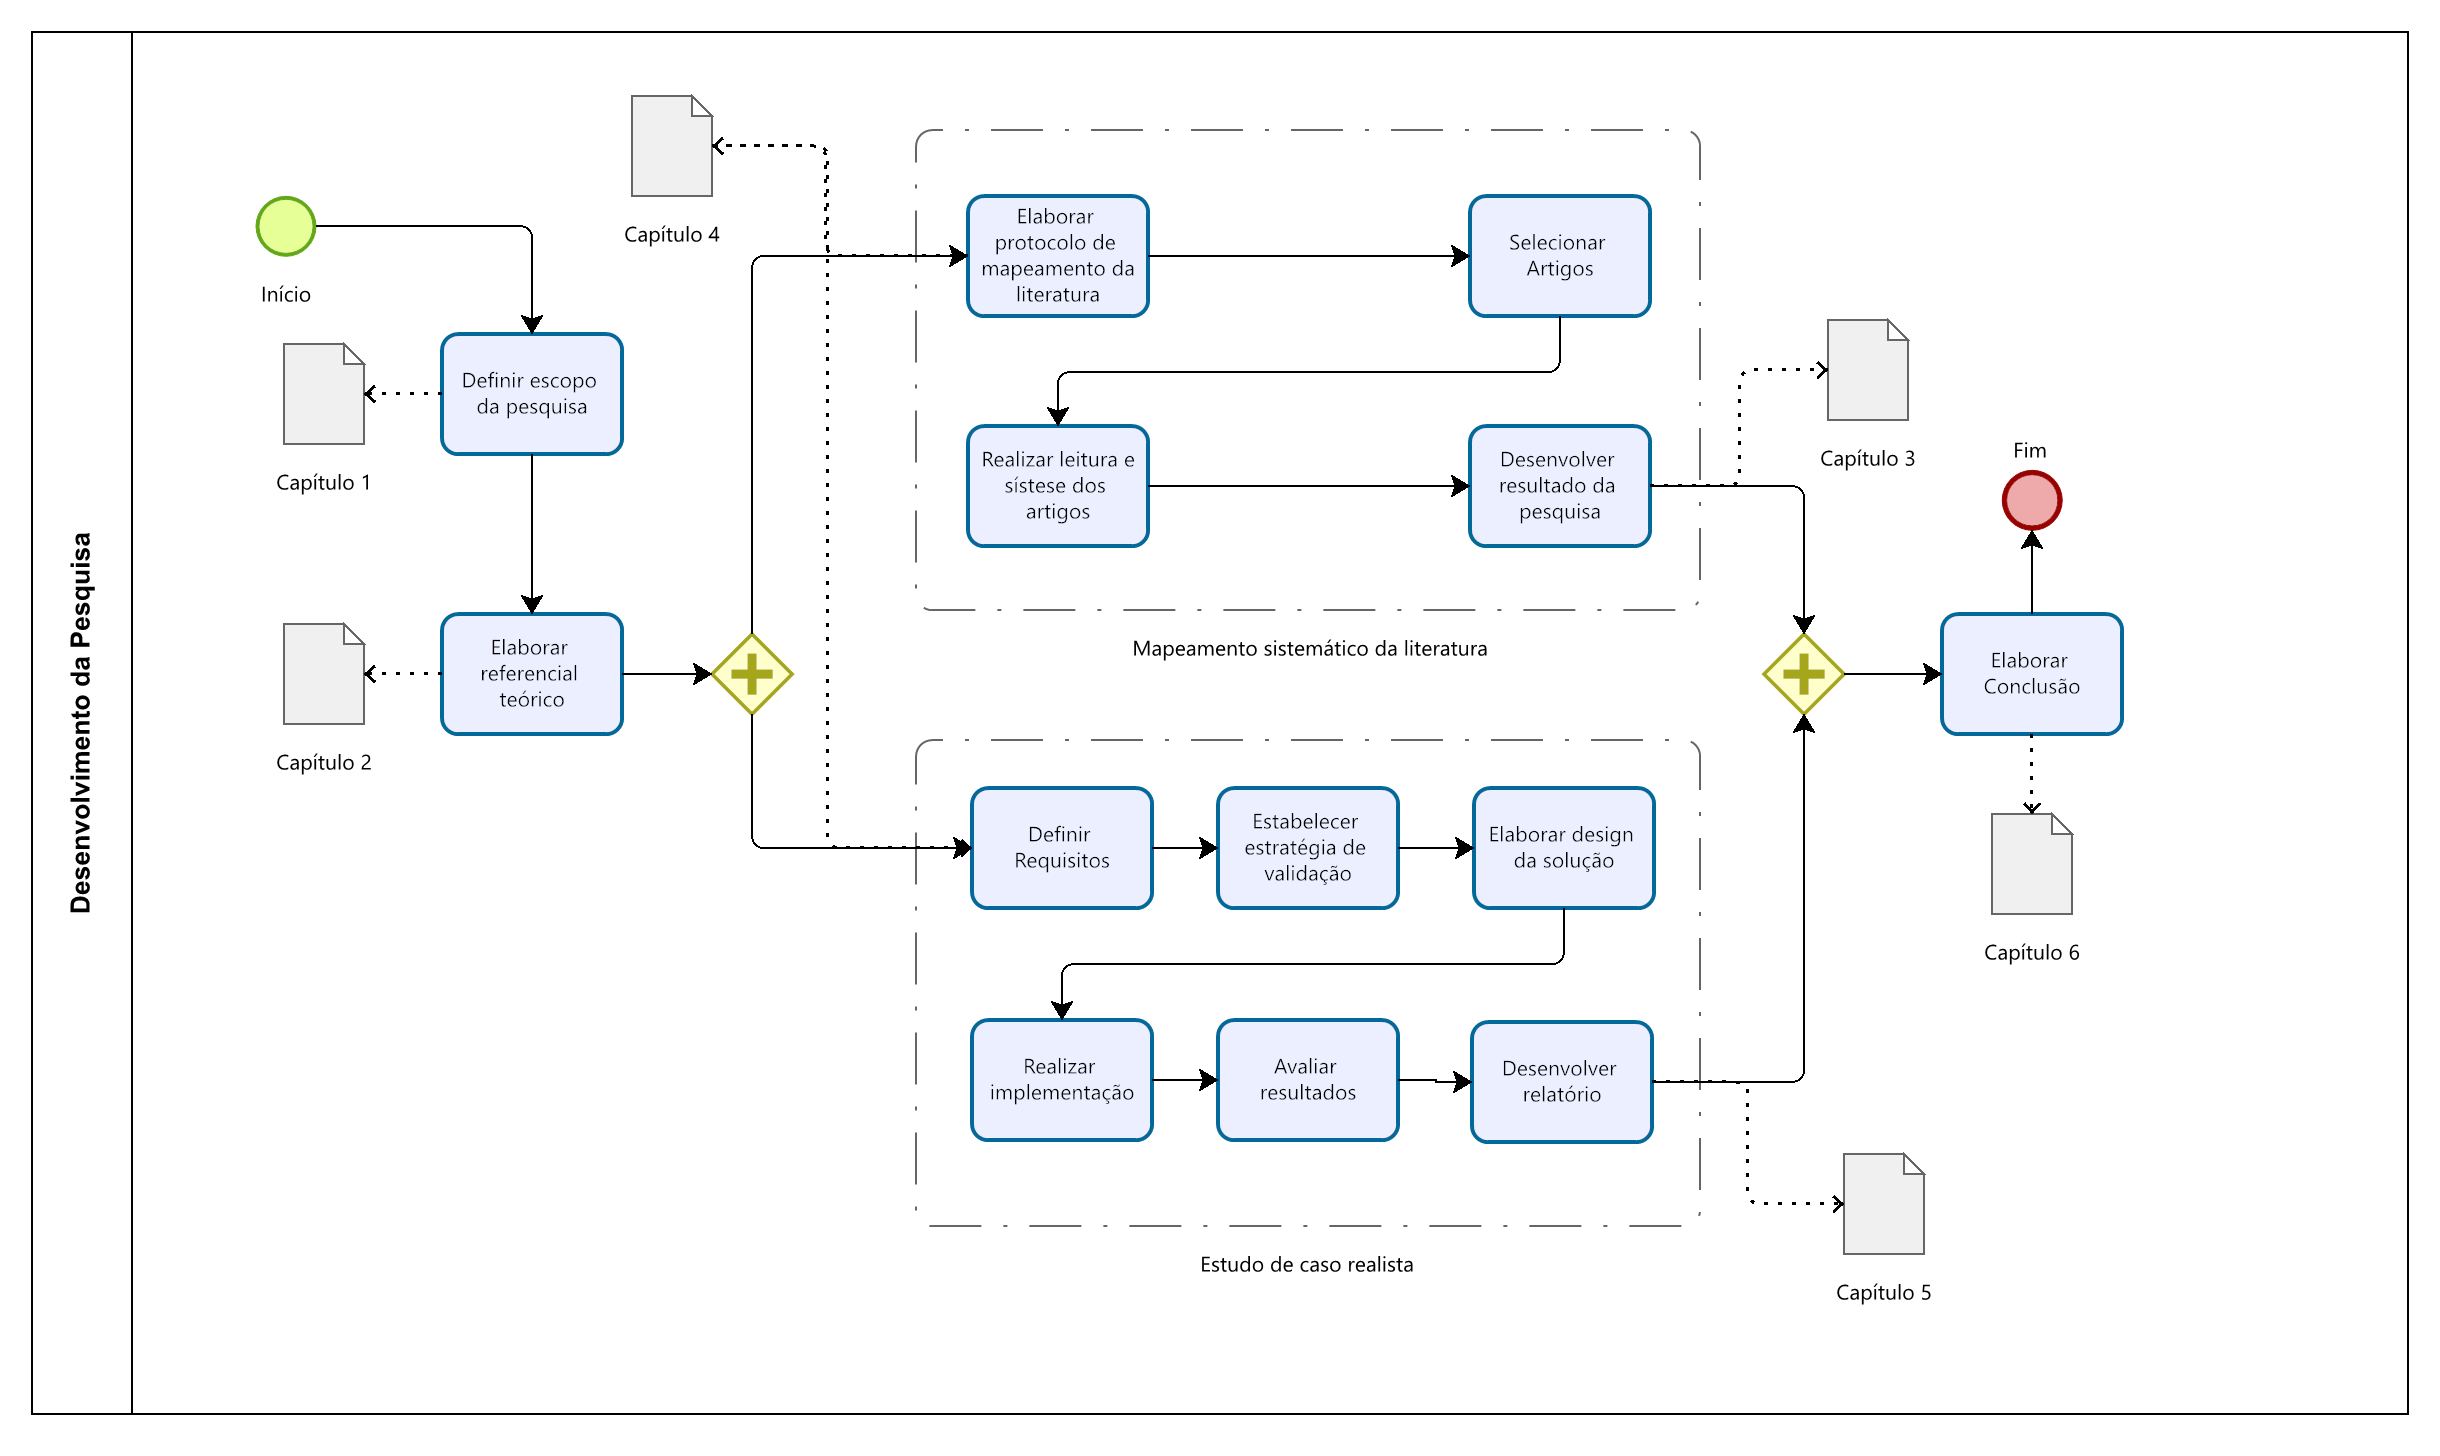
\includegraphics[width=0.9\textwidth]{media/bpmn_metodo_recurso.png}
    \legend{Fonte: o autor}
    \label{fig:metodo_recurso}
\end{figure}

Pode-se observar na \autoref{fig:metodo_recurso} as etapas de execução dessa pesquisa. Inicialmente, o escopo é definido e primeiro capítulo é elaborado. Em seguida, a fundamentação teórica com os conceitos-chave é construída. Posteriormente, se realiza um mapeamento da literatura buscando trabalhos similares. Adicionalmente, um estudo de caso realista com a utilização de microsserviços e diversos conceitos do \acrshort{ddd} é desenvolvido e um relatório é produzido. Por fim, é escrita a conclusão do trabalho.

\section{Mapeamento sistemático da Literatura}
Esta seção apresenta o protocolo de mapeamento sistemático da literatura usado para atingir os objetivos da pesquisa.

\subsection{Problema de pesquisa e contexto}
Nos últimos anos, ocorreu uma mudança paradigmática no desenvolvimento de software \cite{microserviceAdoption}, impulsionada pela necessidade de escalabilidade, flexibilidade e agilidade. Nesse cenário, a arquitetura de microsserviços emergiu como abordagem para construção de grandes sistemas formado por partes independentes e interconectadas entre si. No entanto, uma dos principais desafios dessa arquitetura é a delimitação do escopo de cada serviço \cite{richardson2018microservices}. Assim, \acrfull{ddd} se apresenta como uma importante alternativa para enfrentar essa questão. Assim, esse mapeamento visa compreender como esses dois conceitos estão sendo combinados para potencializar o desenvolvimento de software.

\subsection{Objetivo}
Este mapeamento da literatura visa encontrar artigos contendo estudos de caso, padrões, recomendações e análises da utilização combinada da arquitetura de microsserviços e \acrshort{ddd}. Especificamente sobre os estudos de caso, esta pesquisa está interessada tanto em casos de construção de sistemas de zero, quanto de migração de monólitos existentes. 

\subsection{Justificativa}
Com esse mapeamento da literatura, pretende-se fornecer uma análise valiosa para arquitetos de software, desenvolvedores e pesquisadores sobre os benefícios e desafios da integração de microsserviços com \acrshort{ddd}. Além disso, o conhecimento obtido com esse mapeamento auxiliará na elaboração do estudo de caso realista.

\subsection{Questões de pesquisa}
\label{section:questoes_pesquisa}
\begin{enumerate}
    \item[Q1:] Quais são as principais estratégias para elaboração de sistemas com microsserviços e \acrshort{ddd}?
    \item[Q2:] Quais são os principais desafios na utilização de \acrshort{ddd} como estratégia de delimitação de microsserviços?
    \item[Q2:] Quais são os anti-padrões a serem evitados na utilização de \acrshort{ddd} com microsserviços?
    
\end{enumerate}

\subsection{Estratégia de busca}
Esta seção apresenta a estratégia de buscas de artigos científicos e livros relacionados à pesquisa

\subsubsection{Ferramentas}
\textbf{Periódicos Capes:} É uma ferramenta disponibilizada pelo governo federal para uso de estudantes e pesquisadores. Acessando através da instituição de ensino ou pesquisa, é possível ter acesso completo a uma grande quantidade de artigos científicos publicados em variadas revistas, conferências e universidades. A principal vantagem dessa ferramenta é a possibilidade de ler o conteúdo integral de grande parte das publicações disponíveis. Por outro lado, as expressões de busca atualmente suportadas são bem limitadas.

\textbf{\english{Scopus:}} Trata-se de um ferramenta similar ao Periódicos Capes. No entanto, o \english{Scopus} permite a elaboração de expressões de buscas mais complexas e sofisticadas, servindo para descobrir publicações não detectadas pelas outras plataformas. Além disso, possui um acervo bem mais amplo que o Periódicos Capes. Entretanto, algumas publicações não podem ser vistas na íntegra de forma gratuita.

\textbf{\english{Google Docs:}} Ferramenta desenvolvida pela \english{Google LLC} que permite a criação e edição de documentos de texto. Suas grandes vantagens em relação a ferramentas de outros fornecedores são as avançadas ferramentas de colaboração e a possibilidade de acesso por meio de navegadores \english{web}, sem necessidade de instalação de \english{software} específico.

\textbf{\english{Google Sheets}}: Com as mesmas características e vantagens do \english{Google Docs}, essa ferramenta fornece recursos para elaboração de planilhas de cálculo. É muito útil para realizar análise de dados simples e também visualizar e apresentar dados tabulares.

\subsubsection{Idioma e período}
Como grande parte das publicações na área de computação são em inglês, esta pesquisa utiliza esse idioma para fazer buscas nas ferramentas indicadas.

Além disso, \acrfull{ams} e \acrfull{ddd} são relativamente recentes, as buscas se limitaram a publicações feitas nos últimos 20 anos.

\subsubsection{Termos ou palavras chaves}
Os termos-chave para realização das buscas são: Microsserviço, \acrshort{ddd} e \acrlong{ddd}. Como a busca será feita em inglês, se usará \english{microservice} nas buscas.
\subsubsection{Expressão de busca}
\label{section:string_busca}

\begin{quadro}[H]
\centering

\setlength{\tabcolsep}{0.8em} % for the horizontal padding
\renewcommand{\arraystretch}{1.5}% for the vertical padding
\caption{Expressão de busca utilizada}
\begin{tabular}{|p{4.5in}|}

\hline
Expressão de Busca \\ \hline
\english{( ( TITLE-ABS-KEY ( microservice ) AND TITLE-ABS-KEY ( domain-driven AND design ) ) OR ( TITLE-ABS-KEY ( microservice ) AND TITLE-ABS-KEY ( ddd ) ) )} \\ \hline

\end{tabular}
\label{quad:string_busca}
\fonte{o autor}
\end{quadro}

No \autoref{quad:string_busca}, percebe-se que a expressão de busca pretende retornar todas as publicações que contenham as palavras chaves no título, resumo ou na seção de \english{keywords}.

\subsection{Estratégia de seleção}
A seguir são apresentados critérios para inclusão e exclusão de publicações na pesquisa. Além disso, características para analisar os materiais quanto a qualidade são discutidas. 

\subsubsection{Critérios de inclusão}
\label{section:criterios_inclusao}
\begin{itemize}
    \item Texto completo disponível de forma gratuita pelo portal Periódicos Capes.
    \item Materiais relacionados ao tópico de interesse, ou seja, título ou resumo.
    \item Publicações com ao menos 5 citações.
\end{itemize}

\subsubsection{Critérios de exclusão}
\label{section:criterios_exclusao}
\begin{itemize}
    \item Publicações duplicadas.
    \item Materiais que não dispõem de informação relevante para responder às questões de pesquisa.
\end{itemize}

\subsection{Estratégia para extração de dados e análise}
Para atingir o objetivo do mapeamento da literatura, são filtrados manualmente nos artigos selecionados segundo os critérios de inclusão e exclusão. A partir da listagem reduzida, todas as publicações são lidas de forma integral.
Adicionalmente, todos os gráficos e tabelas nos artigos selecionados são avaliados visando extrair algum dado que permita realizar a comparação entre aspectos quantitativos das estratégias como, tempo de resposta, latência e taxa de transferência.

\subsubsection{Instrumentos de coleta de dados}
Informações qualitativas como recomendações, destaques, conceitos e estudos de casos são registrados em um documento no \english{\href{https://docs.google.com/document/d/1-dXE9_2-CtfDePG9Opkcyipq0F0dcYJ-Z_gbhi_qDhs/edit?usp=sharing}{Google Docs}}. 

Dados quantitativos como taxa de transferência, latência, tempo de processamento são armazenados em uma planilha no \english{\href{https://docs.google.com/spreadsheets/d/1R-PbCisie8QHARzF2rYtDx8UPOWksEeH-6-SEqIOTLg/edit?usp=sharing}{Google Sheets}}. 

\subsubsection{Procedimentos}
A pesquisa é executada seguindo os passos a seguir:
\begin{enumerate}
    \item As expressões de busca citadas são inseridas nas ferramentas mencionadas.
    \item É feito o armazenamento das publicações retornadas em uma \href{https://docs.google.com/spreadsheets/d/1rtH8Jl1EHguqZ4Py2mgV3pab7IQzt72-Sv2S1jPzLsQ/edit?usp=sharing}{planilha de cálculo}.
    \item As publicações retornadas são filtradas conforme os critérios de inclusão e exclusão.
    \item Em cada artigo selecionado, é realizada a extração dos dados relevantes para responder às questões de pesquisa.
    \item Finalmente, são produzidas respostas para questões de pequisa com as informações extraídas das publicações.
\end{enumerate}

\section{Estudo de Caso}
A FAZER
